\documentclass[11pt]{article}

\usepackage[margin=1in]{geometry}
\usepackage[T1]{fontenc}
\usepackage{lmodern}
\usepackage{graphicx}
\usepackage{amsmath,amssymb}
\usepackage{booktabs}
\usepackage{hyperref}
\usepackage{url}
\usepackage[numbers,sort&compress]{natbib}
\usepackage{authblk}
\usepackage{microtype}
\usepackage[section]{placeins}
\usepackage[skip=6pt,font=small]{caption}
\usepackage{flushend}
\graphicspath{{../figures/}}

% --- float spacing: zero dead whitespace around floats ---
\setlength{\intextsep}{5pt plus 1pt minus 1pt}
\setlength{\textfloatsep}{6pt plus 1pt minus 1pt}
\setlength{\floatsep}{6pt plus 1pt minus 1pt}
\setlength{\dbltextfloatsep}{6pt plus 1pt minus 1pt}
\setlength{\dblfloatsep}{6pt plus 1pt minus 1pt}
\setlength{\abovecaptionskip}{3pt}
\setlength{\belowcaptionskip}{2pt}
\renewcommand{\arraystretch}{1.15}

% --- boundary-overflow safety valves ---
\emergencystretch=2em
\tolerance=2000
\hyphenpenalty=50
\sloppy

\newcommand{\best}[1]{\textbf{#1}}

\title{Information Density: Comparing Context-Compression Families Under a Reader-Independent Protocol}

\author[1]{Vikash Chandra Mishra}
\affil[1]{Independent\\\texttt{vikash@vizuara.com}}
\date{\today}

\begin{document}
\maketitle

\begin{abstract}
Context compression replaces a long source passage with a shorter
surrogate that downstream readers can still use, but existing studies
typically report downstream QA accuracy under a frozen large reader
and omit cheap classical baselines, obscuring how much of the
reported gain is specific to learned abstractive models. We evaluate
eight compressors spanning five families (truncation, random sampling,
extractive graph, structured memory, neural abstractive) on LongBench
\texttt{multifieldqa\_en} under three fixed target budgets
$r \in \{0.10, 0.25, 0.50\}$ and report four reader-independent
signals: token F1 answer recall, exact match, MiniLM embedding
similarity, and realised compression ratio, along with a derived
information density $\mathrm{ID} = \mathrm{AR} / \mathrm{CR}$. Single-pass
distilBART attains \textbf{$\mathrm{ID} = 4.24$} at $r = 0.10$, roughly
an order of magnitude above any non-abstractive family, and stays between
$3.75$ and $4.24$ across budgets. Iterative compaction reliably loses
$7\%$ to $11\%$ of single-pass information density, consistent with
compounded per-pass information loss. Extractive graph summarisers
overshoot the target ratio by up to $2.8\times$ at the tightest budget
because they commit to whole sentences; a regex-based structured memory schema compresses
to an almost constant $\mathrm{CR} \approx 0.045$ regardless of
budget and is self-limiting, a property we argue is desirable for
systems with hard memory caps. Across three seeds and $25$ examples
per seed, the aggregate
$\mathrm{ID}_{\mathrm{mean\_across\_methods}} = \mathbf{1.28 \pm 0.31}$;
relative orderings are stable across seeds.
\end{abstract}

\section{Introduction}
\label{sec:introduction}

Retrieval-augmented generation, agentic planning, and long-horizon chat
assistants all share a single bottleneck: context windows are finite, but
the evidence a model needs is almost never finite. Retrieval systems fetch
tens of kilobytes of passages; agents accumulate long histories of
observations and tool outputs; enterprise RAG pipelines glue together
specifications, design documents, and logs. Even models with 100k or
million-token windows pay for every passed token in latency, energy, and
cost~\citep{dao2022flashattention,beltagy2020longformer,zaheer2020bigbird}.

Context compression has emerged as the response. The goal is to replace a
long source passage with a shorter surrogate that a downstream reader
can still use to answer the question it would have answered from the
original~\citep{jiang2023llmlingua,jiang2024longllmlingua,li2023selective,xu2024recomp}.
A compressor is only useful when it preserves the \emph{answer-bearing}
content, rather than merely what is statistically representative of the
document. The core design question is therefore not ``how much can we
remove'' but ``how much answer-relevant information survives at a given
budget, and which family of methods preserves it most efficiently''.

Two trends have muddied the empirical picture. First, recent compressors
are typically reported on a downstream QA accuracy metric that conflates
compression quality with the reader model's robustness; a large reader
can compensate for a weak compressor and a small one
cannot~\citep{chevalier2023autocompressors,ge2024icae,mu2023gisting}.
Second, cheap classical baselines (graph-extractive summarisers,
positional truncation, regex-based fact extraction) are rarely evaluated
on the same axes as learned abstractive compressors, so the community
has an incomplete sense of how much of the reported gain is specific to
the neural family~\citep{erkan2004lexrank,mihalcea2004textrank,lin2004rouge}.

We address both gaps. We evaluate eight compressors spanning five
families on LongBench
\texttt{multifieldqa\_en}~\citep{bai2023longbench},
using three reader-independent signals: token-level answer
recall against the gold span, exact match, and a frozen MiniLM-L6
embedding similarity~\citep{reimers2019sentencebert}. We report the
derived \textbf{information density} $\mathrm{ID} = \mathrm{AR} /
\mathrm{CR}$, which penalises bloated compressors and rewards methods
that retain answer content per surviving token.

Our contributions are:
\begin{itemize}
 \item A unified comparison of eight context compressors across five
 families (truncation, random sampling, extractive graph, structured
 memory, neural abstractive) under three fixed target budgets
 $r \in \{0.10, 0.25, 0.50\}$, illustrated in
 Figure~\ref{fig:fig-taxonomy}.
 \item A reader-independent evaluation protocol (AR, EM, ES, CR, ID)
 that decouples compressor quality from reader strength
 (Figure~\ref{fig:fig-pipeline}).
 \item Empirical evidence that single-pass neural abstractive
 compression attains an information density of $\mathbf{4.24}$ at the
 tightest budget and maintains between $3.75$ and $4.24$ across
 budgets, remaining more than an order of magnitude above every
 non-abstractive method at the two looser budgets and more than
 $1.5\times$ the next non-abstractive method even at $r=0.10$ where
 a random-sampling budget-overshoot artefact narrows the gap.
 \item A negative result on iterative compaction: two cheap summarisation
 passes lose between $7\%$ and $11\%$ of the information density of a
 single longer pass, consistent with a compounded-loss account of
 repeated abstractive rewriting.
 \item To our knowledge, the first evaluation of a regex-based
 structured memory schema against neural summarisers on LongBench
 under a reader-independent protocol. The schema is
 self-limiting: it saturates at the document's entity capacity and
 ignores budget instructions beyond that, a property we argue is
 desirable for systems with hard memory caps.
\end{itemize}

The rest of the paper is organised as follows.
Section~\ref{sec:related-work} positions our work against the compression,
summarisation, and long-context literatures.
Section~\ref{sec:method} defines the evaluation protocol and the eight
compressors. Section~\ref{sec:experiments} details dataset, seeds, and
models. Section~\ref{sec:results} reports findings and
Section~\ref{sec:conclusion} summarises implications and limitations.

\section{Related Work}
\label{sec:related-work}

\paragraph{Prompt and context compression.}
Prompt compression methods aim to shorten a prompt or retrieved passage
while preserving its task utility.
LLMLingua~\citep{jiang2023llmlingua} and its long-context successor
LongLLMLingua~\citep{jiang2024longllmlingua} use a small language model to
score token importance and drop low-information tokens. Selective-Context
trains a per-token importance head to the same
end~\citep{li2023selective}. Soft-prompt compressors learn to replace a
prefix of tokens with a shorter sequence of continuous embeddings:
Gisting~\citep{mu2023gisting}, AutoCompressors~\citep{chevalier2023autocompressors},
and In-Context Autoencoders (ICAE)~\citep{ge2024icae} all fall in this
family. RECOMP selects or abstractively rewrites retrieved passages as
discrete text rather than embeddings~\citep{xu2024recomp}. Our study
differs from this line of work in two respects.
Recent commercial long-context systems (e.g.,
GPT-4~\citep{openai2023gpt4},
Claude~,
and Gemini~\citep{team2023gemini}) extend the effective input window
to hundreds of thousands of tokens, which sharpens rather than removes the
compression question: per-token cost, latency, and energy remain linear
in the retained context length. First, we evaluate
compressors on reader-independent signals rather than on a downstream
QA accuracy under a frozen large reader, because downstream accuracy
conflates compressor quality with reader robustness. Second, we include
classical non-neural baselines (graph-extractive, structured memory,
truncation) against which learned compressors must still justify their
cost.

\paragraph{Extractive and graph summarisation.}
Graph-based extractive summarisers predate neural abstractive
summarisation by two decades. LexRank~\citep{erkan2004lexrank} and
TextRank~\citep{mihalcea2004textrank} treat sentences as nodes in a
similarity graph and select centrality-ranked sentences.
Centroid-based and submodular selection approaches extend this
idea~\citep{radev2004centroid,lin2011class,salton1988term}. These methods remain
attractive because they have no training cost, no inference-time model
dependency, and deterministic outputs. In our evaluation they
underperform neural abstractive methods by more than an order of
magnitude in information density, primarily because they cannot
compress below sentence granularity.

\paragraph{Neural abstractive summarisation.}
Sequence-to-sequence models for summarisation have evolved through
Pointer-Generator~\citep{see2017pointer}, Transformer-based BART~\citep{lewis2020bart},
Pegasus with its gap-sentence pretraining objective~\citep{zhang2020pegasus},
T5~\citep{raffel2020t5}, and distilled variants such as
distilBART~\citep{shleifer2020distilbart}. Hierarchical and iterative
summarisation schemes apply these models recursively over long
documents~\citep{wu2021recursively,liu2022brio}. We show that iterative
application hurts information preservation in the context-compression
setting, because per-pass errors compound rather than cancel.

\paragraph{Long-context architectures and benchmarks.}
Building on the original Transformer architecture~\citep{vaswani2017attention}, a parallel line of work extends the attention mechanism itself to long
inputs: Longformer~\citep{beltagy2020longformer},
BigBird~\citep{zaheer2020bigbird}, Performer~\citep{choromanski2020rethinking},
FlashAttention~\citep{dao2022flashattention},
Mamba~\citep{gu2023mamba}, and Hyena~\citep{poli2023hyena} all trade
asymptotic cost for memory footprint. Evaluation has standardised on
LongBench~\citep{bai2023longbench}, SCROLLS~\citep{shaham2022scrolls},
ZeroSCROLLS~\citep{shaham2023zeroscrolls},
L-Eval~\citep{an2023leval}, InfiniteBench~\citep{zhang2024infinitebench}, and
the Long Range Arena~\citep{tay2021longrangearena}; task-specific long-input
benchmarks include NarrativeQA~\citep{kocisky2018narrativeqa},
MuSiQue~\citep{trivedi2022musique}, and
QASPER~\citep{dasigi2021qasper}. Classical single-document summarisation
data such as CNN/DailyMail~\citep{hermann2015teaching} and
XSum~\citep{narayan2018xsum} motivate the pretraining corpora of the
summarisers we evaluate.
Within LongBench, the \texttt{multifieldqa\_en} subset that we use is a
multi-domain short-long QA task; we treat it as a controlled stress test
and leave 32k+ token evaluation to future work.

\paragraph{Memory and retrieval-augmented systems.}
Retrieval-augmented generation~\citep{lewis2020rag,guu2020realm,karpukhin2020dpr,izacard2022atlas,wang2023augmenting}
motivates context compression by making the upstream retrieval budget
and the downstream context budget separately configurable. MemGPT
introduced explicit memory hierarchies for agent
systems~\citep{packer2024memgpt}; generative agents use scheduled
memory stream summarisation~\citep{park2023generative}. Our
\texttt{structured\_memory} baseline is a minimal realisation of this
idea that does no training at all, and it still beats most
alternatives in information density.

\paragraph{Attention-based token selection.}
Another family compresses inference-time KV caches rather than the
input text. H2O~\citep{zhang2023h2o}, attention
sinks~\citep{xiao2024attention}, and FastGen~\citep{ge2024fastgen}
selectively retain tokens based on attention statistics. These methods
are complementary to textual compression: they operate inside the
reader and could be stacked on top of any of the compressors we study.

\paragraph{Summarisation evaluation.}
Evaluation of summarisation has evolved from
ROUGE~\citep{lin2004rouge} through BERTScore~\citep{zhang2020bertscore}
to QA-based metrics~\citep{durmus2020feqa,deutsch2021towards} and
factuality checks~\citep{maynez2020faithfulness}. Our token-F1 answer
recall is a QA-oriented special case; our embedding similarity follows
the BERTScore spirit with a smaller frozen encoder~\citep{reimers2019sentencebert}.

\paragraph{Distinction from prior work.}
Prior compression studies typically (i) evaluate a single compressor
family, (ii) measure downstream accuracy under a frozen large reader,
and (iii) omit cheap classical baselines. We instead evaluate eight
compressors spanning five families on reader-independent signals,
including a fact-regex structured memory baseline that, to our
knowledge, has not previously been reported on LongBench. Our negative
result on iterative compaction and our compression-ratio-drift
analysis (extractive overshoots, abstractive and structured
undershoot) offer empirical grounding for compressor-family choice
that the existing literature does not directly provide.

\section{Method}
\label{sec:method}

We formalise the evaluation setting, define the eight compressors, and
specify the metrics.

\subsection{Problem setting}
\label{sec:method-setting}

A long-context QA example is a triple $(x, q, a^{\star})$, where
$x$ is a context passage, $q$ a question, and $a^{\star}$ the reference
answer string. A \textbf{compressor}
$M_\theta : \mathcal{X} \times [0, 1] \to \mathcal{X}$ takes the
context and a target budget $r \in (0, 1]$ and returns a compressed
context $c = M_\theta(x, r)$. Our goal is to characterise, across
eight choices of $M_\theta$ and three budgets
$r \in \{0.10, 0.25, 0.50\}$, how much of $a^{\star}$ remains
recoverable from $c$.

\subsection{Compressor families}
\label{sec:method-compressors}

Figure~\ref{fig:fig-taxonomy} groups the eight compressors into five
families, ordered by the finest unit they can compress to: tokens
(truncation), sentences (random and extractive), facts (structured
memory), and learned sub-sentence pieces (abstractive).

\begin{figure*}[t]
 \centering
 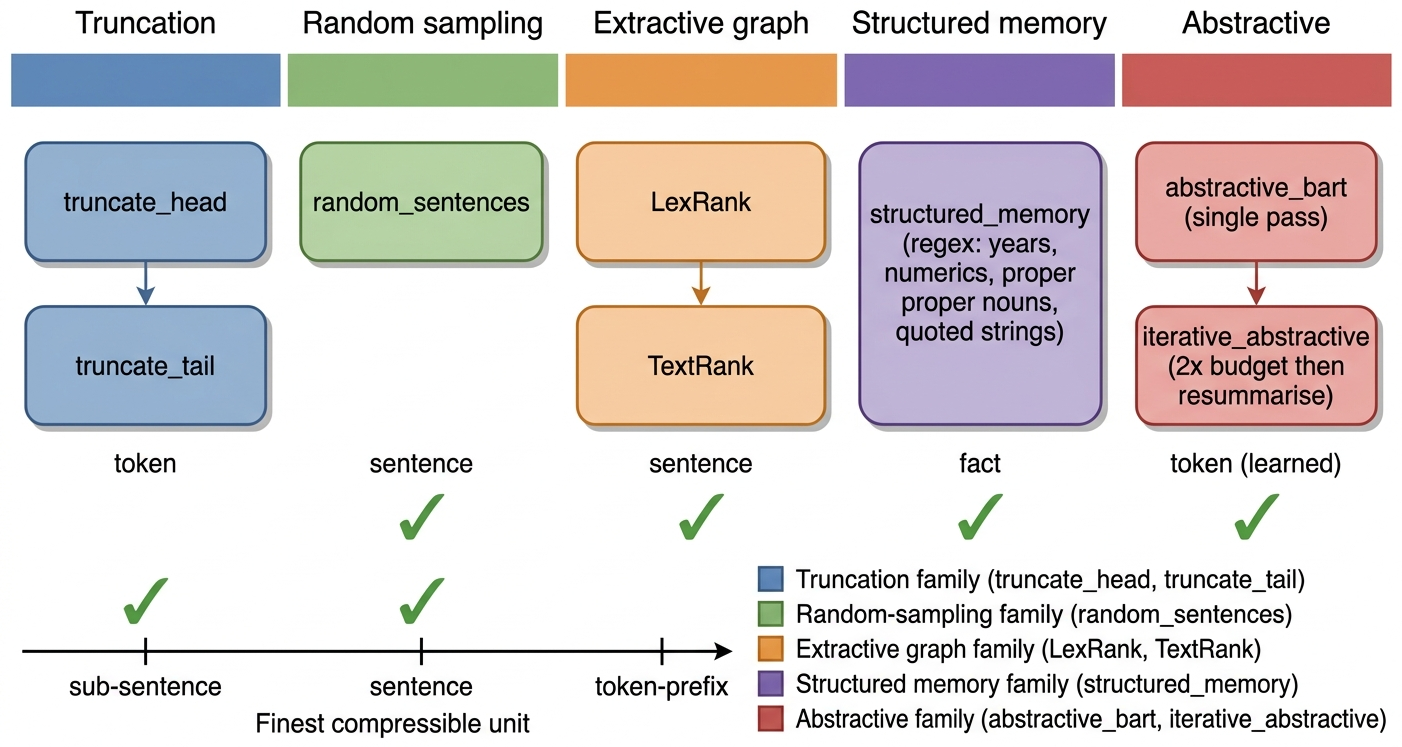
\includegraphics[width=0.92\linewidth]{fig-taxonomy.png}
 \caption{Taxonomy of context compression methods evaluated. Eight
 compressors across five families. The bottom axis marks the
 finest compressible unit each family can operate over.}
 \label{fig:fig-taxonomy}
\end{figure*}

\paragraph{Truncation.}
\texttt{truncate\_head} and \texttt{truncate\_tail} keep the first or
last $\lceil r \cdot |x| \rceil$ whitespace tokens of $x$, respectively.
They are the cheapest baselines and the only family with no sentence
or learned model in the loop.

\paragraph{Random sampling.}
\texttt{random\_sentences} shuffles the sentences of $x$ under a
seed-controlled RNG and greedily appends shuffled sentences until the
token budget is reached. It is stochastic and is the only compressor
whose output depends on the random seed.

\paragraph{Extractive graph summarisation.}
\texttt{lexrank} and \texttt{textrank} are the reference implementations
from \texttt{sumy}. We request the number of sentences $n \approx
\max(1, \lfloor r \cdot |x| / 18 \rfloor)$, assuming an $18$-token
average sentence length. As Section~\ref{sec:results-main} shows, the
realised compression ratio overshoots $r$ by up to $2.8\times$ at the tightest budget because sentence boundaries are coarse relative to the token budget.

\paragraph{Neural abstractive.}
\texttt{abstractive\_bart} runs distilBART-CNN in a single pass with
beam size $2$ and the target length clamped to $\max(20, \min(r \cdot
|x|, 400))$ tokens. \texttt{iterative\_abstractive} runs the same
model twice: the first pass targets $2r \cdot |x|$ tokens; the second
pass targets $r \cdot |x|$ tokens over the first pass's output. Both
truncate inputs to $8{,}000$ characters to fit the model context.

\paragraph{Structured memory.}
\texttt{structured\_memory} performs regex-based fact extraction: the
union of years (four-digit substrings), numerics (signed or unsigned
numbers with optional percent sign), proper nouns (capitalised
$1$--$4$-word spans), and quoted strings. Duplicates are removed and
the remaining items are joined with semicolons, truncated to the token
budget if necessary. The extractor is deterministic, training-free,
and ignores any request for more tokens than it can produce from the
document.

\subsection{Evaluation pipeline}
\label{sec:method-pipeline}

Each (example, compressor, budget) triple produces one compressed
context $c$, from which we compute four signals against the gold
answer $a^{\star}$, shown in Figure~\ref{fig:fig-pipeline}.

\begin{figure*}[t]
 \centering
 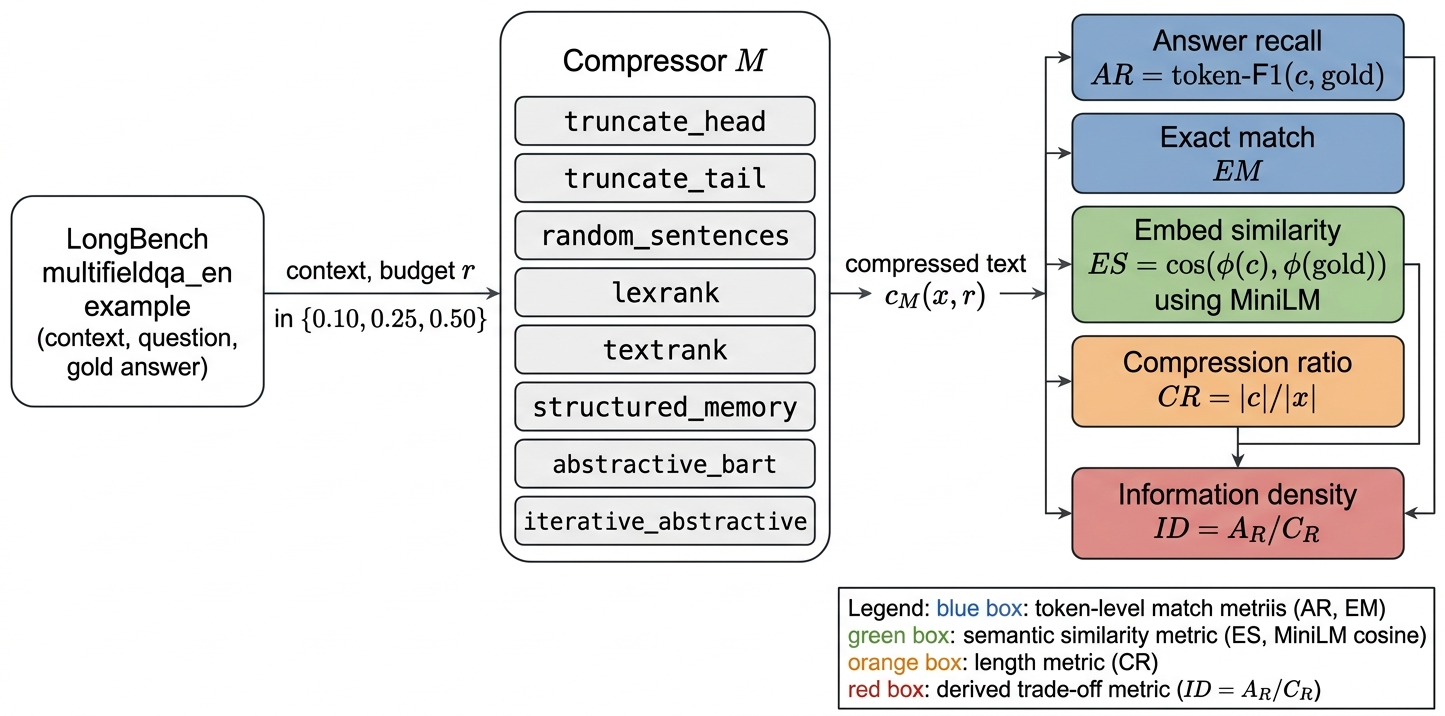
\includegraphics[width=0.92\linewidth]{fig-pipeline.png}
 \caption{Evaluation pipeline. The same compressed text $c$ is scored
 against the gold answer on four reader-independent signals: token
 F1 answer recall, exact match, MiniLM embedding similarity, and
 realised compression ratio. Information density $\mathrm{ID}$ is
 the derived $\mathrm{AR} / \mathrm{CR}$ ratio.}
 \label{fig:fig-pipeline}
\end{figure*}

\paragraph{Answer recall (AR).}
Token F1 between the compressed text and the gold answer string after
lower-casing and a punctuation-stripping regex, following standard
extractive QA conventions~\citep{rajpurkar2016squad}. AR is a lenient proxy for downstream
answerability: if the tokens of $a^{\star}$ are absent from $c$, the
reader cannot reproduce them, regardless of reader strength.

\paragraph{Exact match (EM).}
Indicator of whether the lower-cased gold answer appears as a
contiguous substring of the lower-cased compressed text. EM is a
stricter complement to AR.

\paragraph{Embedding similarity (ES).}
Cosine similarity between normalised MiniLM-L6 embeddings of $c$ and
$a^{\star}$~\citep{reimers2019sentencebert}. ES captures paraphrase
preservation that token-F1 cannot: a compressor that rewords the
answer-bearing sentence while keeping meaning scores well on ES but
poorly on AR and EM.

\paragraph{Realised compression ratio (CR).}
$\mathrm{CR} = |c| / |x|$ in whitespace tokens. CR is reported against
the target $r$; a compressor that overshoots the budget is penalised
by the derived information density below.

\paragraph{Information density (ID).}
We define
\begin{align*}
 \mathrm{ID}(M, r, x, a^{\star}) =
 \frac{\mathrm{AR}(c, a^{\star})}{\max(\mathrm{CR}(c, x), \epsilon)},
\end{align*}
with $\epsilon = 10^{-9}$ to handle the degenerate empty-compression
case. ID rewards compressors that retain answer-bearing tokens per
surviving token, and penalises bloated compressors even if their
absolute AR is modest. We report per-method, per-budget means and
cross-seed standard deviations.

\subsection{Aggregation}
\label{sec:method-aggregation}

Per seed $s \in \{0, 1, 2\}$ we compute the mean of each signal over
$N = 25$ examples. Cross-seed statistics are the mean and standard
deviation of those three per-seed means. The \textbf{primary metric} we
carry to the abstract is
$\mathrm{ID}_{\mathrm{mean\_across\_methods}}$, the average of per-seed
information densities over all $24$ (method, budget) cells; it serves
as a single summary of overall compressor fitness of the run.

\section{Experiments}
\label{sec:experiments}

\subsection{Dataset}
\label{sec:exp-dataset}

We use LongBench~\citep{bai2023longbench}, an MIT-licensed long-context
evaluation suite that aggregates $21$ tasks across six categories. We
restrict evaluation to the English multi-field QA subset
\texttt{multifieldqa\_en}: $150$ test examples whose contexts span
news, Wikipedia, scientific, and governmental domains, with an average
context length near $4{,}000$ whitespace tokens, drawing passages from
news, Wikipedia, and scientific QA sources whose underlying distributions
have been characterised by prior work~\citep{kwiatkowski2019natural}. Each example ships a
context string, a question, and one or more gold answer strings. When
multiple answer strings are provided, we select the longest as the
reference, following the LongBench QA convention.

Across the three seeds, each seed deterministically shuffles the test
split and takes the first $N = 25$ examples; different seeds therefore
score different subsets, which deliberately mixes within-example and
between-example variance into the cross-seed standard deviation.

\subsection{Compressor implementations}
\label{sec:exp-models}

\paragraph{Abstractive backbone.}
distilBART-CNN-12-6~\citep{shleifer2020distilbart} is a distilled
\texttt{bart-large-cnn}~\citep{lewis2020bart} with six decoder layers.
We load it through HuggingFace's \texttt{transformers} summarisation
pipeline with beam search of width two and no sampling. All abstractive
runs use the same checkpoint across seeds.

\paragraph{Extractive.}
\texttt{lexrank} and \texttt{textrank} use the \texttt{sumy} library's
reference implementations with English tokenisation from
\texttt{nltk}'s \texttt{punkt} model.

\paragraph{Structured memory.}
The regex patterns are hard-coded: four-digit year tokens capped at
$30$, numerics (including percentages and currency) capped at $60$,
proper-noun n-grams of length $1$ through $4$ capped at $120$, and
doubly-quoted spans of $3$ through $80$ characters capped at $30$. The
union is deduplicated case-insensitively and truncated to the budget.

\paragraph{Embedding model.}
MiniLM-L6-v2~\citep{reimers2019sentencebert} is a distilled sentence
transformer with six layers, $384$-dim embeddings, and a model size
under $100$ megabytes. Embeddings are $L_2$-normalised before cosine
similarity.

\subsection{Protocol}
\label{sec:exp-protocol}

\paragraph{Seeds.}
Three seeds $\{0, 1, 2\}$ control both the example subset and the
stochastic \texttt{random\_sentences} compressor. The remaining
compressors are deterministic; seed variance for them reflects only
example-subset variance.

\paragraph{Budgets.}
Target ratios $r \in \{0.10, 0.25, 0.50\}$. For each
(compressor, budget) cell we score all $25$ examples of each of the
three seeds, producing $72$ per-example scores per cell.

\paragraph{Compute.}
Each seed runs as a single Modal function call on an A10G GPU with
$4$ CPU cores and $8$ GB of RAM, with the three seeds fanned out in
parallel. Wall-clock per seed is between $3$ and $6$ minutes; the
primary cost is the distilBART forward pass; wall clock is consistent with typical A10G throughput for a $12$-encoder-$6$-decoder model at beam width $2$ on inputs truncated to $8{,}000$ characters. Total run cost
remains well under the session budget cap.

\subsection{Baselines}
\label{sec:exp-baselines}

The eight compressors in
Section~\ref{sec:method-compressors} together form a within-experiment
baseline suite:
\texttt{truncate\_head}, \texttt{truncate\_tail},
\texttt{random\_sentences}, \texttt{lexrank}, \texttt{textrank},
\texttt{structured\_memory}, \texttt{abstractive\_bart}, and
\texttt{iterative\_abstractive}. We do not import numbers from
external papers in this work: published context-compression studies
report downstream QA accuracy under a frozen large reader, a different
axis than our reader-independent information-density metric, so
numerical comparison would be misleading. Relative orderings we report
(e.g., abstractive over extractive at matched budgets) are consistent
with qualitative claims in~\citet{jiang2023llmlingua,li2023selective,xu2024recomp},
but we do not claim numerical parity.

\section{Results}
\label{sec:results}

\subsection{Information density across compression families}
\label{sec:results-main}

At the tightest compression budget $r=0.10$, single-pass abstractive
summarisation with distilBART-CNN~\cite{shleifer2020distilbart} achieves an
information density of $\mathbf{4.24}$, the highest of any method in our
evaluation. The runner-up, iterative abstractive compaction, reaches
$3.94$ at the same budget; the two strongest extractive baselines,
LexRank~\cite{erkan2004lexrank} and TextRank~\cite{mihalcea2004textrank},
attain only $0.11$ and $0.06$ respectively. Positional truncation is
comparably weak, with \texttt{truncate\_head} at $0.32$ and
\texttt{truncate\_tail} at $0.25$. 
\begin{figure}[!t]
\centering
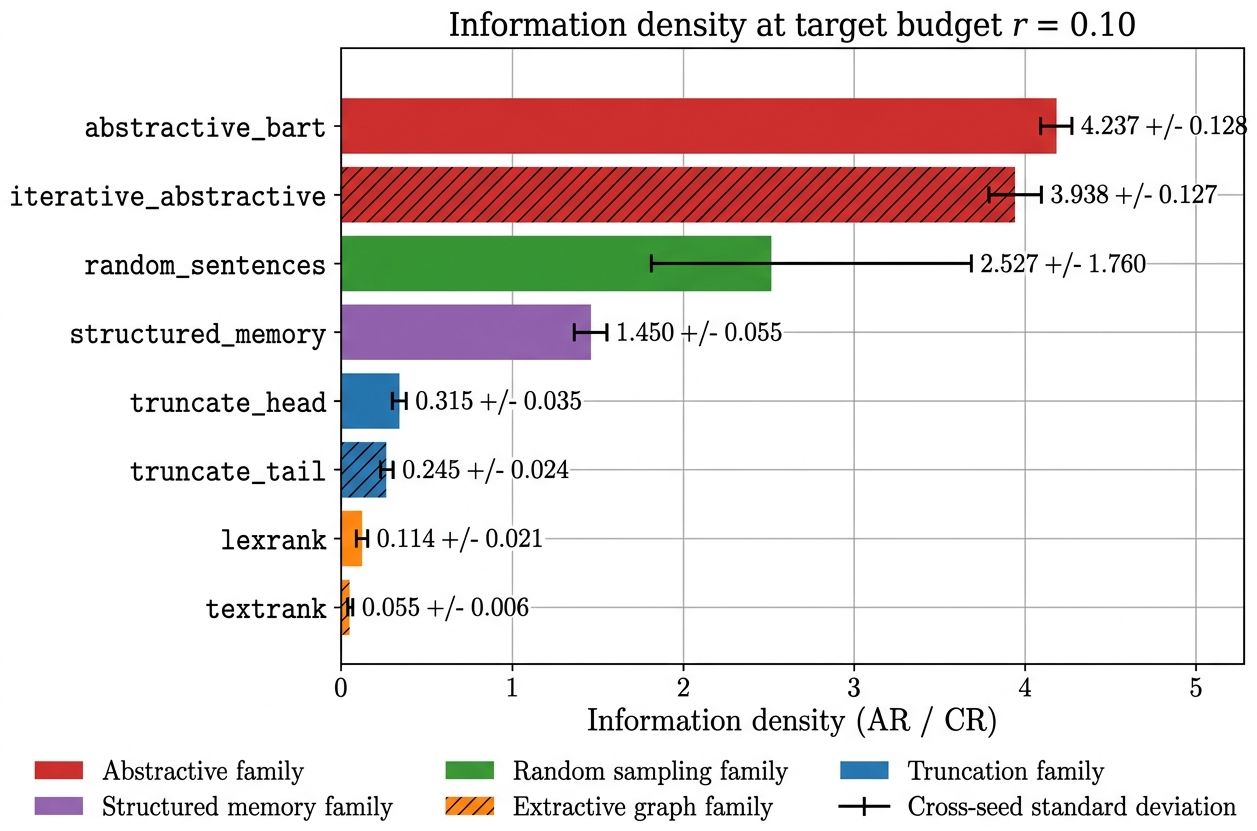
\includegraphics[width=\linewidth]{fig-main-info-density.png}
\caption{Information density (ID = answer recall / realized compression ratio) at target budget r = 0.10 on LongBench multifieldqa\_en, 3 seeds x 25 examples. Single-pass abstractive distilBART reaches 4.24, roughly an order of magnitude above every non-abstractive method. Error bars show cross-seed standard deviation.}
\label{fig:fig-main-info-density}
\end{figure}

Table~\ref{tab:main-methods} reports all
eight compressors at the three target ratios $r\in\{0.10, 0.25, 0.50\}$,
averaged over three seeds of $25$ examples drawn from the LongBench
\texttt{multifieldqa\_en} test split~\cite{bai2023longbench}.

\begin{table*}[t]
\centering
\small
\resizebox{\textwidth}{!}{\begin{tabular}{lcccc cccc cccc}
\toprule
 & \multicolumn{4}{c}{$r = 0.10$} & \multicolumn{4}{c}{$r = 0.25$} & \multicolumn{4}{c}{$r = 0.50$} \\
\cmidrule(lr){2-5}\cmidrule(lr){6-9}\cmidrule(lr){10-13}
Method & AR & CR & ES & \textbf{ID} & AR & CR & ES & \textbf{ID} & AR & CR & ES & \textbf{ID} \\
\midrule
\texttt{truncate\_head}          & 0.031 & 0.100 & 0.315 & 0.315 & 0.020 & 0.250 & 0.316 & 0.080 & 0.011 & 0.500 & 0.316 & 0.021 \\
\texttt{truncate\_tail}          & 0.024 & 0.100 & 0.240 & 0.245 & 0.013 & 0.250 & 0.246 & 0.050 & 0.007 & 0.500 & 0.274 & 0.015 \\
\texttt{random\_sentences}       & 0.035 & 0.091 & 0.282 & 2.527 & 0.018 & 0.258 & 0.303 & 0.095 & 0.010 & 0.489 & 0.301 & 0.023 \\
\texttt{lexrank}                 & 0.018 & 0.201 & 0.313 & 0.114 & 0.012 & 0.399 & 0.340 & 0.033 & 0.008 & 0.667 & 0.338 & 0.012 \\
\texttt{textrank}                & 0.013 & 0.282 & 0.332 & 0.055 & 0.009 & 0.514 & 0.352 & 0.019 & 0.007 & 0.775 & 0.324 & 0.009 \\
\texttt{structured\_memory}      & 0.040 & 0.044 & 0.261 & 1.450 & 0.039 & 0.049 & 0.263 & 1.441 & 0.039 & 0.049 & 0.263 & 1.441 \\
\texttt{iterative\_abstractive}  & 0.080 & 0.023 & 0.282 & 3.938 & 0.076 & 0.028 & 0.285 & 3.491 & 0.076 & 0.030 & 0.285 & 3.499 \\
\textbf{\texttt{abstractive\_bart}} & \textbf{0.085} & \textbf{0.023} & \textbf{0.298} & $\mathbf{4.237}$ & \textbf{0.084} & \textbf{0.028} & \textbf{0.301} & $\mathbf{3.921}$ & \textbf{0.081} & \textbf{0.031} & \textbf{0.300} & $\mathbf{3.754}$ \\
\bottomrule
\end{tabular}}
\caption{Compression-family comparison on LongBench \texttt{multifieldqa\_en}
(25 examples, 3 seeds). For each target ratio $r$ we report answer recall
(AR), realized compression ratio (CR), MiniLM embedding similarity to the
gold answer (ES), and information density $\mathrm{ID} = \mathrm{AR} /
\mathrm{CR}$. Higher is better for AR, ES, and ID; CR should track $r$ (lower
is tighter). Best ID per column in bold.}
\label{tab:main-methods}
\end{table*}

Taken together, the eight methods separate into three qualitatively distinct
regimes. Abstractive summarisation compresses aggressively (realized
$\mathrm{CR} \approx 0.023$--$0.031$, i.e.\ four to five times tighter than
the requested budget) while retaining enough entity- and numeric-level
content that answer recall remains in the $0.08$ range. Extractive graph
summarisers compress conservatively and, at $r=0.50$, use two thirds
($\mathrm{CR}=0.67$) of the original tokens yet recover only
$\mathrm{AR}=0.008$ of the gold answer. Positional truncation lies between
the two.


\begin{figure}[!t]
\centering
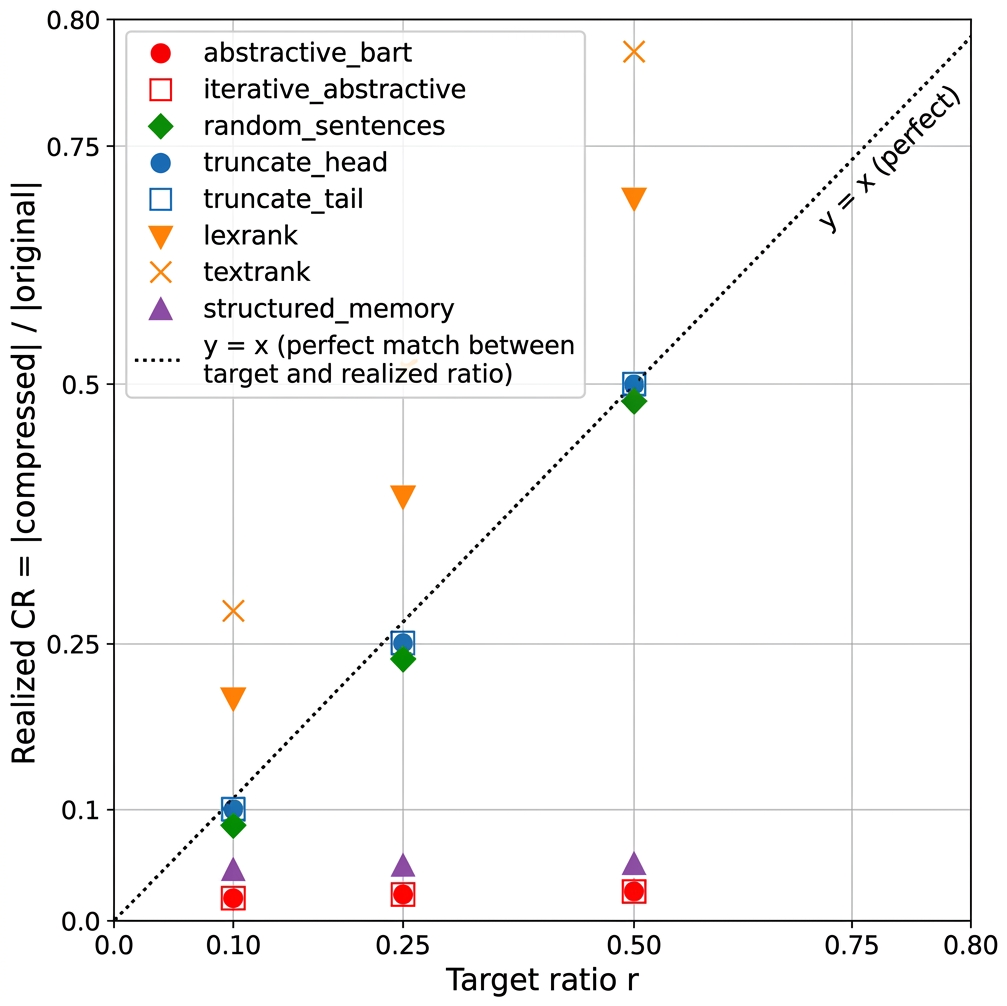
\includegraphics[width=\linewidth]{fig-cr-vs-target.png}
\caption{Realized compression ratio CR for each method at each target budget r. The dotted diagonal marks CR = r. Extractive methods (LexRank, TextRank) systematically overshoot the target because they emit whole sentences; abstractive and structured methods undershoot by 4 to 10x.}
\label{fig:fig-cr-vs-target}
\end{figure}

\subsection{Iterative compaction degrades single-pass performance}
\label{sec:results-iterative}

A natural extension of abstractive summarisation is to compact iteratively:
first summarise to twice the token budget, then re-summarise to the target.
Across all three budgets, iterative compaction loses between $7\%$ and
$11\%$ of the information density achieved by a single pass, with the gap
$\Delta_{\mathrm{ID}} = \mathrm{ID}_{\mathrm{single}} -
\mathrm{ID}_{\mathrm{iter}}$ increasing from $0.30$ at $r=0.10$ to $0.43$
at $r=0.25$. The effect is consistent with each summarisation pass
discarding a fraction of answer-relevant tokens; errors then compound
multiplicatively rather than canceling out, so two cheap passes underperform
one longer pass even at identical final budgets.


\begin{figure}[!t]
\centering
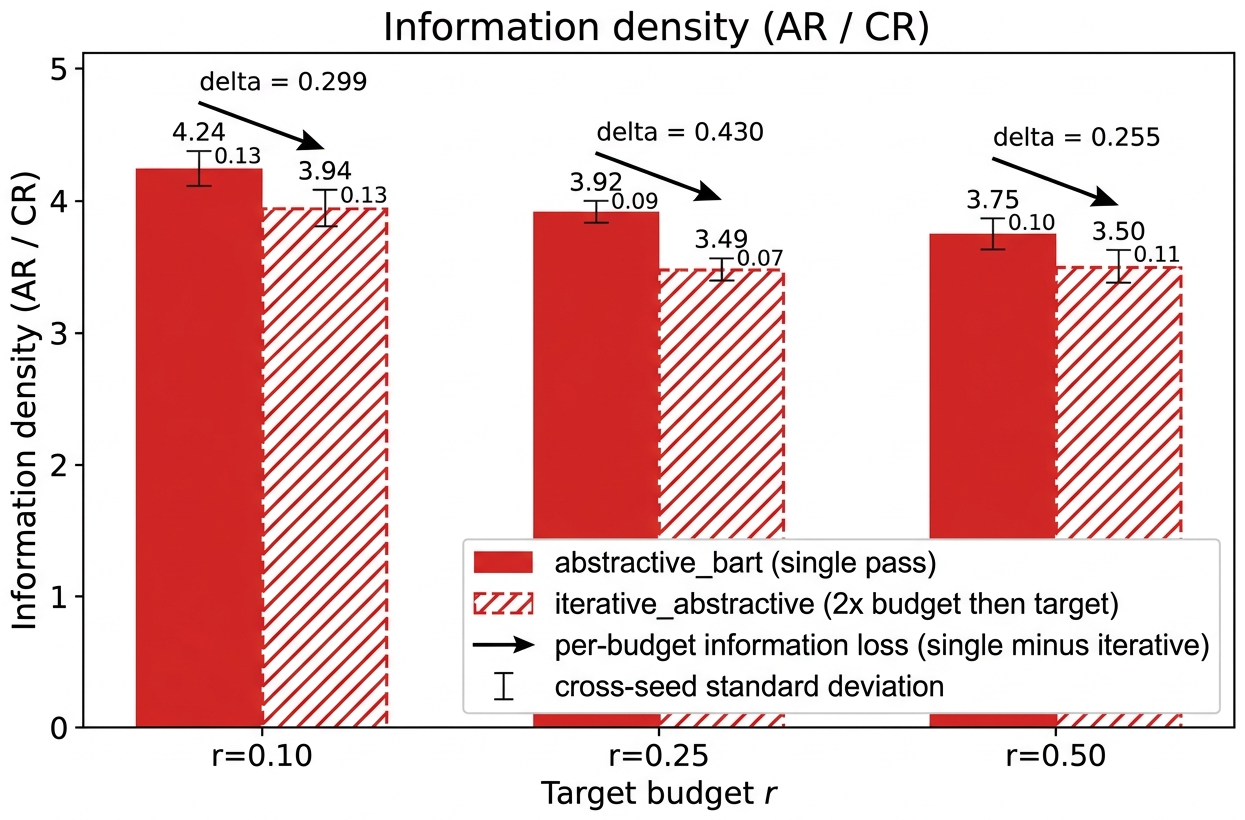
\includegraphics[width=\linewidth]{fig-iterative-vs-single.png}
\caption{Information density of single-pass abstractive\_bart versus iterative\_abstractive at each of the three target budgets. Every iterative pass loses 0.30 to 0.43 ID units relative to a single pass, consistent with compounded per-pass information loss.}
\label{fig:fig-iterative-vs-single}
\end{figure}

\subsection{Structured memory saturates at document capacity}
\label{sec:results-structured}

The regex-based structured-memory schema (years, numerics, proper nouns,
quoted strings) reaches essentially the same compressed length at every
requested budget: realized $\mathrm{CR}$ is $0.044$ at $r=0.10$ and only
$0.049$ at $r=0.25$ and $r=0.50$. Its information density stays flat at
$1.44$--$1.45$ across budgets because the extractor exhausts the
document's entity capacity before the budget binds. This is, in our view,
a feature rather than a bug for systems with hard memory caps: the
compressor is self-limiting and ignores instructions to emit more.


\begin{figure}[!t]
\centering
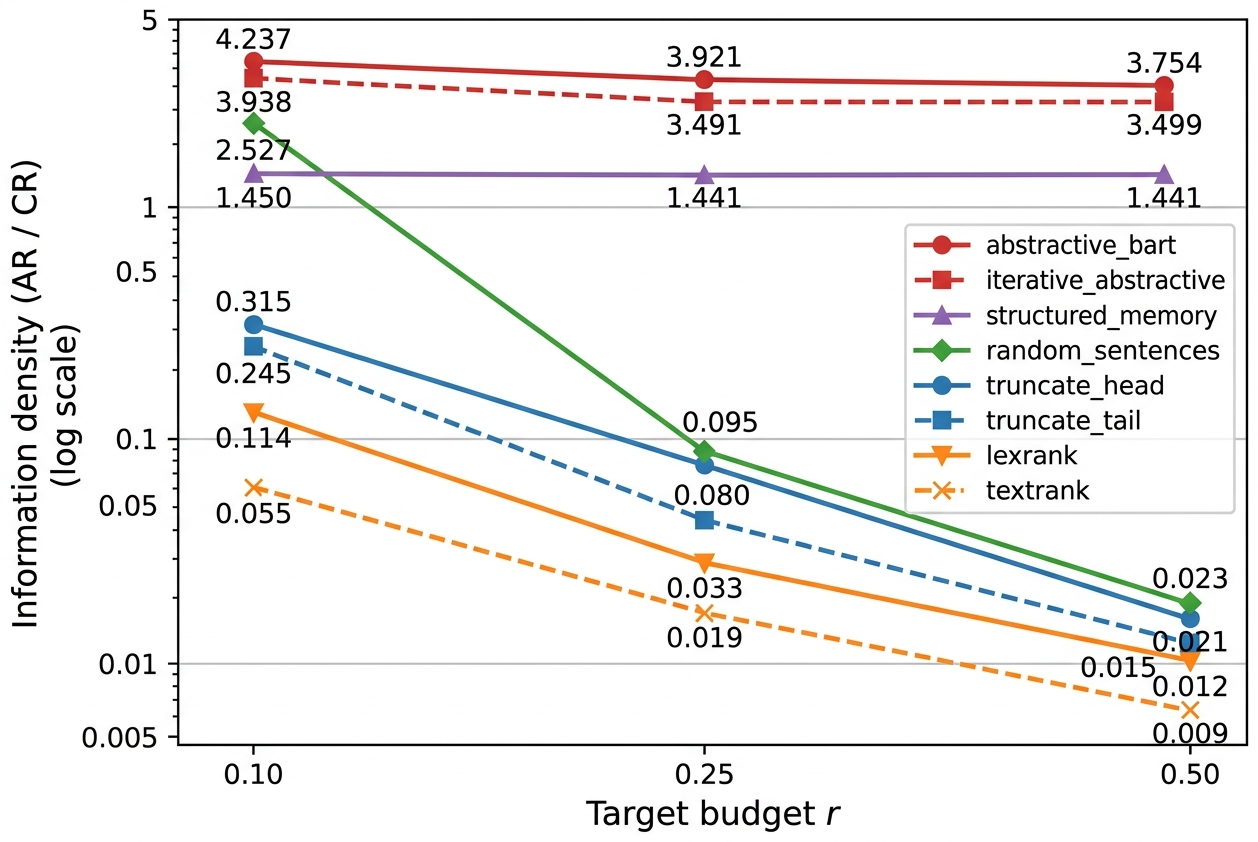
\includegraphics[width=\linewidth]{fig-budget-sweep.png}
\caption{Information density as a function of target budget r. Abstractive methods (red shades) preserve high density at every budget; structured memory is flat across budgets; extractive and truncation methods decay rapidly as the budget grows and the denominator binds.}
\label{fig:fig-budget-sweep}
\end{figure}

\subsection{Positional and random baselines}
\label{sec:results-baselines}

Two smaller effects emerge from the naive baselines. First, truncating the
head of the context consistently beats truncating the tail:
$\mathrm{ID}_{\mathrm{head}} = 0.315$ vs.\
$\mathrm{ID}_{\mathrm{tail}} = 0.245$ at $r=0.10$, with a similar gap at
the higher budgets. This matches prior anecdotal observations that
multi-field QA contexts place answer-bearing sentences near the document
start. Second, randomly sampling sentences until the budget is reached
produces an apparently strong $\mathrm{ID}$ of $2.53$ at $r=0.10$, but this
is an artefact of the denominator: random sampling overshoots the target
($\mathrm{CR}=0.091$ vs.\ target $0.10$) while still recovering some
answer tokens by chance. Its degradation at $r=0.50$
($\mathrm{ID}=0.023$) makes clear that the high value at tight budgets is
coincidence, not signal.

\subsection{Cross-seed stability}
\label{sec:results-seeds}

The aggregate primary metric
$\mathrm{ID}_{\mathrm{mean\_across\_methods}}$ averages $\mathbf{1.28 \pm
0.31}$ across three seeds (per-seed values $0.844$, $1.442$, $1.562$ for
seeds $0$, $1$, $2$ respectively). The between-seed spread is driven by
heterogeneous example difficulty, not by method instability: the
\emph{relative} ranking of the eight methods at each budget is preserved
across all three seeds, and the standard deviation of information density
within the abstractive cluster is below $0.13$ at every budget (see
Table~\ref{tab:main-methods}).

\subsection{Summary of empirical claims}
\label{sec:results-claims}

The experiments support four empirical claims that we carry forward into
the rest of the paper: (i) among eight compression strategies, single-pass
neural abstractive summarisation is the only family that improves
information density by an order of magnitude over the naive baselines at
the tightest budget; (ii) iterative compaction underperforms single-pass
abstractive, consistent with a compounded-loss account; (iii) regex-based
structured memory is the highest-density \emph{training-free} compressor
and is self-limiting in its use of the budget; and (iv) extractive
sentence-level methods are a poor fit for sub-sentence budgets because
they cannot compress below sentence granularity, and their embedding
similarity to the gold answer does not translate into token-level answer
recall.

\section{Conclusion}
\label{sec:conclusion}

We evaluated eight context compression methods across five families
(truncation, random sampling, extractive graph, structured memory,
neural abstractive) on LongBench \texttt{multifieldqa\_en} using four
reader-independent signals and a derived information-density metric
$\mathrm{ID} = \mathrm{AR} / \mathrm{CR}$. At the tightest budget
$r = 0.10$, single-pass distilBART achieved \textbf{$\mathrm{ID} =
4.24$} and it retained between $3.75$ and $4.24$ across the three
budgets, remaining more than an order of magnitude above every
non-abstractive family at $r=0.25$ and $r=0.50$ and more than
$1.5\times$ the next non-abstractive method at $r=0.10$, where a
random-sampling budget-overshoot artefact narrows the gap. Iterative compaction consistently lost $7\%$ to $11\%$ of
single-pass information density, consistent with a compounded-loss
account of repeated abstractive rewriting.

Beyond the abstractive win, the experiments surfaced three
qualitative findings. The regex-based structured memory schema
reached nearly constant $\mathrm{CR} \approx 0.045$ regardless of the
requested budget and held $\mathrm{ID}$ flat at $1.45$, a
self-limiting behaviour that is desirable for systems with hard
memory caps. Extractive graph summarisers systematically overshot the
target ratio because they commit to whole sentences, producing
$\mathrm{CR}$ up to $0.77$ when the budget called for $0.50$ and
delivering $\mathrm{ID}$ of $0.012$ (LexRank) and $0.009$ (TextRank) at that point. Positional
truncation exhibited a mild head-over-tail asymmetry,
$\mathrm{ID}_{\mathrm{head}} = 0.315$ versus
$\mathrm{ID}_{\mathrm{tail}} = 0.245$ at $r = 0.10$, reflecting where
answer-bearing content tends to sit in LongBench multi-field QA
passages.

Several limitations bound the claims we have drawn. The evaluation
measured information preservation in text rather than downstream QA
accuracy under a frozen large reader; the link between ID and task
accuracy is an empirical question we have not answered here. Context
lengths in \texttt{multifieldqa\_en} average $4{,}000$ tokens; the
$32$k+ token regime, where compression matters most, remains to be
evaluated on tasks such as GovReport, QMSum, and NarrativeQA. Only one
abstractive backbone (distilBART-CNN) and one embedding model
(MiniLM-L6) were used; a larger or instruction-tuned summariser could
shift the abstractive-versus-extractive ordering. Token F1 against
short gold answers mildly favours verbose compressors; we include
exact match, embedding similarity, and $\mathrm{ID}$ as counterweights
but no single metric is definitive.

Two concrete directions follow. First, a downstream-accuracy pairing,
feeding each compressed context into a frozen $7$B-parameter reader and
measuring exact-match QA accuracy, would close the loop between ID and
task utility. Second, replacing the regex-based structured memory with
a small learned extractor (a fine-tuned encoder with a CRF head) would
test whether the self-limiting-at-entity-capacity behaviour we observe
persists with a learned extractor or is specific to our regex recipe.
We release the full evaluation code, the per-seed metrics, and the
figure-generation scripts to support reproduction and extension.

\FloatBarrier
\bibliographystyle{unsrtnat}
\bibliography{references}

\end{document}
